\section{Results from First Science Run}
\par
In this section limits are placed on the elastic EFT operator couplings using data from the LZ's first science run (SR1).
The vanilla WIMP region of interest is considered here rather than an extended one as extending the region of interest would have resulted in a delay to this thesis.
An analysis for SI and SD dark matter interactions have already been performed in this recoil energy range \cite{lz_ws_sr1_ref} and discussed in \cite{marisarthurs_thesis_ref} as such only a limited summary of the SR1 is presented here.
Additionally all plots shown in this section except the signal models and limits originate from collaborators from LZ and are not the authors own creation.

\subsection{Overview of SR1}
\par
SR1 ran for a total of 116 days from 23 December 2021 to 18 April 2022.
During this period, several breaks occurred for both calibration runs and system maintenance reducing the data set down to 89 live days.
For the entire period of SR1 the detector was in a stable state.
The length of time running was driven by a requirement to demonstrate physics capability and so only ran until the sensitivity to SI interactions was comparable to previous experiments.
In that sense, SR1 was more of an engineering run.
As such no blinding or salting of the data set was performed, as with any new detector there are unexpected features that are best understood by being able to see them.
In order to mitigate bias from this decision, analysis cuts were developed in side bands.


\subsection{TPC Calibration}
\par
The spacial variation in $S1$ and $S2$ were corrected using primarily internal sources which are naturally dispersed throughout the detector volume.
${}^{83m}$Kr and ${}^{131m}$Xe were used for this along with injected tritium (injected as tritiated methane CH$_3$T).
Energy calibrations were performed with the internal sources as well and also used ${}^{129m}$Xe which is monoenergetic at higher energies outside of the region considered here.
$g_1$ was determined to be 0.114$\pm$0.002 phd/photon and $g_2$ as 47.1$\pm$1.1 phd/electron.
The size of a single electron was measured as 57.6$\pm$1.9 phd/electron which gives an electron extraction efficiency of 80.5$\pm$3.7\%.
For calibrating the detector model, NR events were produced produced using the DD neutrons and AmLi, whilst ER events were produced using tritium.
The detector response was tuned to these measurements which are shown in \autoref{fig:sr1_tpc_calibration} along with the ER and NR bands.
\begin{figure}
    \centering
    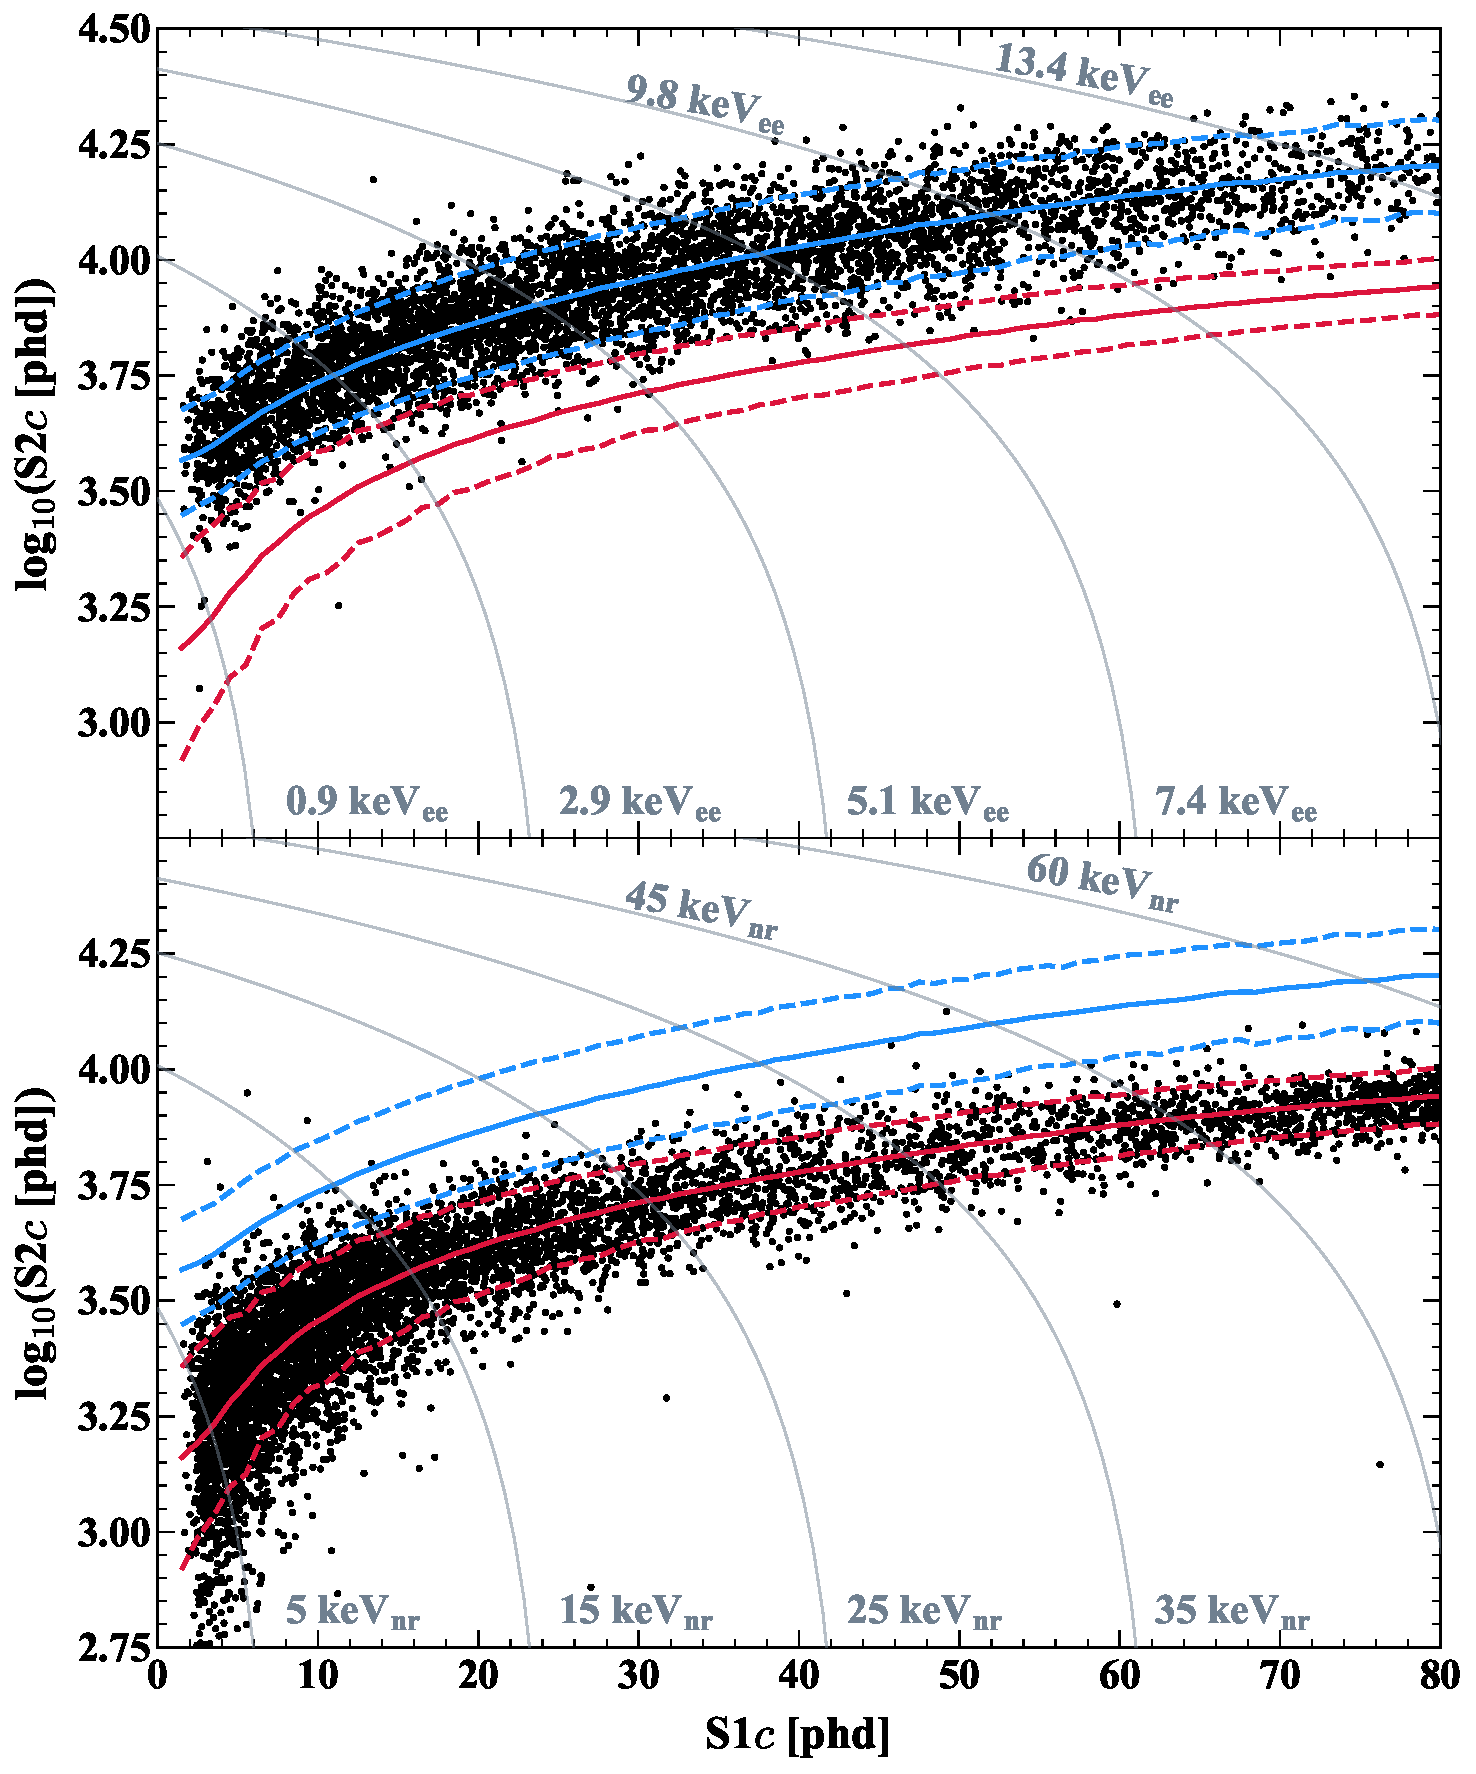
\includegraphics[width=10cm]{Figures/EFT/All_SR1_Plots/SR1WS_calOnly_0629_twoPanel.pdf}
    \caption{Calibration of ER and NR bands, shown in blue and red respectively.
             The solid line is the median and the dashed are the 10\% and 90\% quantiles.
             \textbf{Top:} ER events produced by $\beta$-decays from injected CH$_3$T.
             \textbf{Bottom:} NR events produced by DD neutrons.
             }
    \label{fig:sr1_tpc_calibration}
\end{figure}

\subsection{Analysis Cuts}
\par
In addition to the core-cuts that remove scatters that are inconsistent with dark matter that have been previously discussed, a multitude of other cuts were developed.
They fall broadly into three categories: live time, S2-based cuts and S1-based cuts.
These three, along with the core cuts are briefly discussed below.

\paragraph{live time cuts}
The live time cuts are named as such as they have a large adverse affect on the amount of data that is uncharacteristic due to the high rate of pulses observed.
The two most significant cuts were an electron-train cut and a hot spot cut, together removing 35\% of the livetime.
After a large S2 event, a period of a sustained high rate is observed. 
This is due to electrons attaching to impurities and then being released at some later time, causing a delayed extraction and an elevated rate after the S2.
Single photons are also observed after the same event which is thought to be from delayed fluorescence.
The removal of time after an S2 until the detector rate settles corresponds to 29.8\% of live day loss.
Occasionally hot spots appeared in the TPC due to electron emission from the grids. 
These periods of time lasted approximately an hour at a time and reduced the live time by 6.6\%.
There were several other cuts in this category which combined livetime by a future 1\%.

\paragraph{S2 cuts}
A suite of cuts were developed to remove S2s which did not look like an S2 should if it had originated from a LXe scatter.
These targeted accidental events.

\paragraph{S1 cuts}


developed a hot spot where 

\paragraph{Core cuts}
Select events which have only scattered once, ``single scatter". An event is a single scatter in the TPC if the energy-weighted standard deviation of the deposits is less than the detector resolution. This is taken to be $\sigma_r <$ 3.0 cm and $\sigma_z <$ 0.2 cm.
Select events where the recoil energy is in the range expected from a WIMP scatter and set on S1$_c$, S2 (uncorrected). This is cut is dependent upon which model of dark matter we are using. Here S1$_c$ must be less than 500 phd and have at least a 3-fold coincidence in the TPC PMTs. S2 must be greater than 415, the value required for at least 5 emitted electrons. This electron requirement is to ensure that the S2 size is large enough for position reconstruction.
The inner volume, or fiducial volume of the TPC is taken, removing events near the edges. The FID is defined as a cylinder extended from the centre of the TPC to 4 cm from the TPC walls, 2 cm above the cathode grid, and 13 cm below the gate grid. This inner volume contains 5.6 tonnes of LXe, meaning that there is 1.4 tonnes of xenon used for self-shielding.
TPC scatters where there is a time-coincident deposit in either of the veto detectors are removed. In the Skin detector the signal must be within 800 $\mu$s of the TPC scatter and be at least 3 phd in size. In the OD the deposit must be at least 200 keV in size and within 500 $\mu$s of the TPC scatter. This OD selection was chosen to maintain consistency with \cite{LZ_projected_sensitivity_paper_ref} with an older simulation framework.



\subsection{Background Model}
\par



\paragraph{${}^{37}$Ar}
A source not considered in the projected sensitivity, ${}^{37}$Ar is 

\cite{lz_argon37_ref}.

\paragraph{Accidentals}





\begin{figure}[!htbp]%
\centering
\begin{tikzpicture}
\centering
    \begin{axis}[
            ylabel={Efficiency},
            xlabel={Recoil Energy (keV$_{NR}$)},
            width=15cm,
            height=8cm,
            ymin=0.0, ymax=1.2,
            xmin=0, xmax=70,
            ]
        \addplot[black, only marks,]
            table [x=Energy, y=Efficiency]
            {Data/HENR/sr1_ws/nr_efficiency.dat};
    \end{axis}
\end{tikzpicture}
    \caption{SR1 search data after all cuts.}
    \label{fig:henr_ws_sr1_nr_efficiency}
\end{figure}

\subsection{Result}

\begin{figure}[!htbp]%
\centering
\begin{tikzpicture}
\centering
    \begin{axis}[
            ylabel={log${}_{10}$(S2$_c$ [phd])},
            xlabel={S1 [phd]},
            width=15cm,
            height=8cm,
            ymin=2.75, ymax=4.5,
            xmin=0, xmax=80,
            ]
            
        \addplot[gray, opacity = 0.5, fill=gray]
            table [x=x, y=y]
            {Data/HENR/sr1_ws/sr1_data/beta_band_95.dat};
        \addplot[gray, fill=gray]
            table [x=x, y=y]
            {Data/HENR/sr1_ws/sr1_data/beta_band_68.dat};
    
        \addplot[green, opacity = 0.5, fill=green]
            table [x=x, y=y]
            {Data/HENR/sr1_ws/sr1_data/b8_band_95.dat};
        \addplot[green, fill=green]
            table [x=x, y=y]
            {Data/HENR/sr1_ws/sr1_data/b8_band_68.dat};
            
        \addplot[red, ]
            table [x=x, y=y]
            {Data/HENR/sr1_ws/nr_band.dat};    
        \addplot[red, dashed]
            table [x=x, y=high]
            {Data/HENR/sr1_ws/nr_band.dat};     
        \addplot[red, dashed]
            table [x=x, y=low]
            {Data/HENR/sr1_ws/nr_band.dat}; 
            
        \addplot[black, only marks,]
            table [x=S1c, y=log_10S2c]
            {Data/HENR/sr1_ws/ws_data.dat};
            
        \addplot[orange]
            table [x=x, y=y]
            {Data/HENR/sr1_ws/sr1_data/ar37_band_95.dat};
        \addplot[orange]
            table [x=x, y=y]
            {Data/HENR/sr1_ws/sr1_data/ar37_band_68.dat};
    \end{axis}
\end{tikzpicture}
    \caption{SR1 search data after all cuts.}
    \label{fig:henr_ws_sr1_events}
\end{figure}


\begin{table}[]
    \centering
    \begin{tabular}{c|c|c}
        Background Component     & Expected Events    & Fit Result  \\ \hline
        $\beta$ decays + Det. ER & 218 $\pm$ 36       & 222 $\pm$ 16 \\
        $\nu$ ER                 & 27.3 $\pm$ 1.6     & 27.3 $\pm$ 1.6 \\
        ${}^{127}$Xe             & 9.2 $\pm$ 0.8      & 9.3 $\pm$ 0.8 \\
        ${}^{124}$Xe             & 5.0 $\pm$ 1.4      & 5.2 $\pm$ 1.4 \\
        ${}^{136}$Xe             & 15.2 $\pm$ 2.4     & 15.3 $\pm$ 2.4 \\
        ${}^{8}$B CE$\nu$NS      & 0.15 $\pm$ 0.01    & 0.15 $\pm$ 0.01 \\
        Accidentals              & 1.2 $\pm$ 0.3      & 1.2 $\pm$ 0.3 \\
        ${}^{37}$Ar              & [0, 291]           & 52.1${}^{+9.6}_{-8.9}$ \\
        neutrons                 & 0.0${}^{+0.2}$     & 0.0${}^{+0.2}$
    \end{tabular}
    \caption{Primary backgrounds that need to be considered for an EFT search}
    \label{tab:sr1_ws_lz_backgrounds}
\end{table}


Despite using a smaller parameter space, the sheer increase in the exposure offered by LZ places world-leading limits on every operator coupling.